\subsection{Widgets}
\label{subsec:widgets}
Zur Entwicklung einer \ac{gui} werden grafische Komponenten benötigt. Qt verwendet dafür sogenannte \emph{Widgets}. Widgets sind grafische
Komponenten um die Benutzeroberfläche zu gestalten. Ein Beispiel für eine solche Komponente wäre ein Button, welcher in der Sektion
\emph{\nameref{subsec:programmierbeispiel}} als \emph{btnExit} vorkam.
\newline
\newline
Die Widgets, die Qt zur Verfügung stellt sind in einer großen Klassenhierarchie zusammengesetzt
und diese Hierarchie könnte sich wie folgt dargestellt werden:
\newpage
\begin{figure}[h]
    \centering
    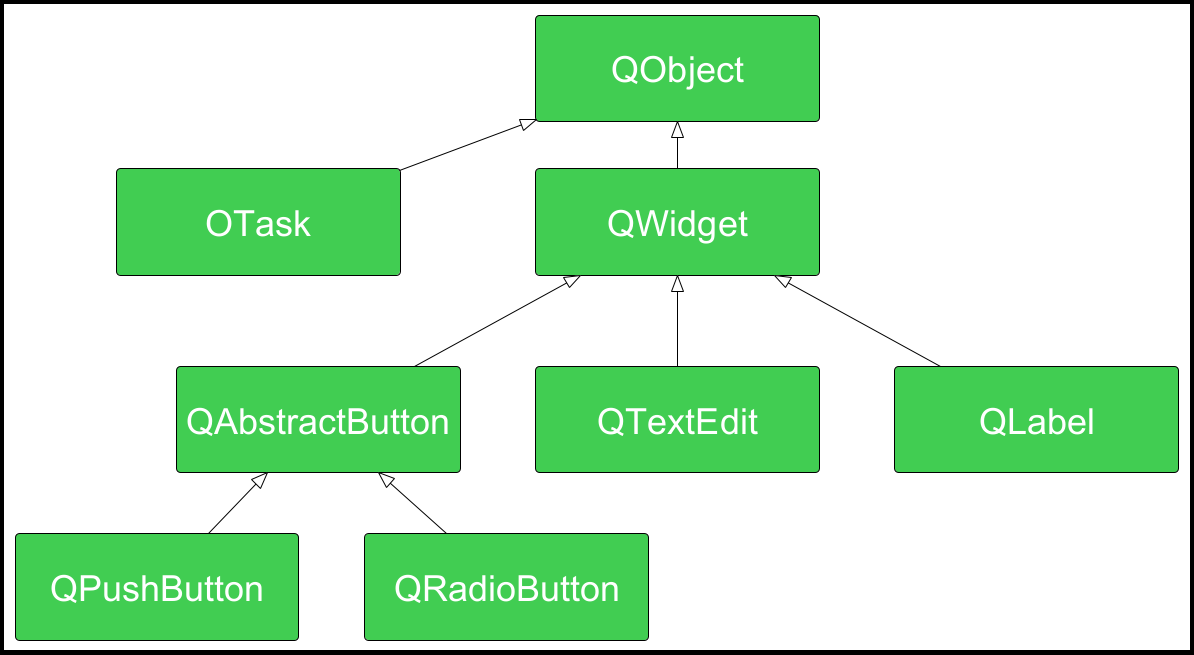
\includegraphics[width=\textwidth, center]{StandDerTechnik/qtWidgetClassHierachie}
    \caption[Qt Widgets Klassenhierachie]{Qt Widgets Klassenhierarchie
    \cite{GettingStartedQt}[vgl.]}
    \label{img:qtWidgetClassHierachie}
\end{figure}

Als Basisklasse ist ganz oben in der Klassenhierarchie die \emph{QObject} Klasse. Diese
enthält unter anderem den Signal- und Slot-Mechanismus. Auf diesen soll später noch genauer
eingegangen werden.
Weitergehend werden Widgets, die gemeinsame Funktionalitäten aufweisen zusammen gruppiert. Diese
Verhalten ist bei \emph{QPushButton} und \emph{QRadioButton} erkennbar. Beide Widgets sind
Buttons, die sich Teilweise die gleichen Eigenschaften und Funktionen teilen
\cite{GettingStartedQt}[vgl.].
